%!TEX program=xelatex

% 碰到Windows版本提示Fandol字体,可以在命令行中以管理员权限执行:tlmgr update -self -all
%\documentclass[review]{cvpr}
\documentclass[final]{cvpr}

\usepackage[UTF8]{ctex}

%\usepackage{cvpr}
\usepackage{times}
\usepackage{epsfig}
\usepackage{graphicx}
\usepackage{amsmath}
\usepackage{amssymb}
\usepackage{subfigure}
\usepackage{overpic}
% \usepackage{float}
\usepackage{stfloats}
\usepackage{enumitem}
\usepackage[noend]{algpseudocode}   %
\usepackage{setspace}   %
\setenumerate[1]{itemsep=0pt,partopsep=0pt,parsep=\parskip,topsep=5pt}
\setitemize[1]{itemsep=0pt,partopsep=0pt,parsep=\parskip,topsep=5pt}
\setdescription{itemsep=0pt,partopsep=0pt,parsep=\parskip,topsep=5pt}


\usepackage[pagebackref=true,breaklinks=true,colorlinks,bookmarks=false]{hyperref}


%\cvprfinalcopy % *** Uncomment this line for the final submission

\def\cvprPaperID{159} % *** Enter the CVPR Paper ID here
\def\confYear{CVPR 2020}
\def\httilde{\mbox{\tt\raisebox{-.5ex}{\symbol{126}}}}

\newcommand{\cmm}[1]{\textcolor[rgb]{0,0.6,0}{CMM: #1}}
\newcommand{\todo}[1]{{\textcolor{red}{\bf [#1]}}}
\newcommand{\alert}[1]{\textcolor[rgb]{.6,0,0}{#1}}

\newcommand{\IT}{IT\cite{98pami/Itti}}
\newcommand{\MZ}{MZ\cite{03ACMMM/Ma_Contrast-based}}
\newcommand{\GB}{GB\cite{conf/nips/HarelKP06}}
\newcommand{\SR}{SR\cite{07cvpr/hou_SpectralResidual}}
\newcommand{\FT}{FT\cite{09cvpr/Achanta_FTSaliency}}
\newcommand{\CA}{CA\cite{10cvpr/goferman_context}}
\newcommand{\LC}{LC\cite{06acmmm/ZhaiS_spatiotemporal}}
\newcommand{\AC}{AC\cite{08cvs/achanta_salient}}
\newcommand{\HC}{HC-maps }
\newcommand{\RC}{RC-maps }
\newcommand{\Lab}{$L^*a^*b^*$}
\newcommand{\mypara}[1]{\paragraph{#1.}}

\graphicspath{{figures/}}

% Pages are numbered in submission mode, and unnumbered in camera-ready
%\ifcvprfinal\pagestyle{empty}\fi
\setcounter{page}{1}


\renewcommand{\figref}[1]{图\ref{#1}}
\renewcommand{\tabref}[1]{表\ref{#1}}
\renewcommand{\equref}[1]{式\ref{#1}}
\renewcommand{\secref}[1]{第\ref{#1}节}
\def\abstract{\centerline{\large\bf 摘要} \hspace*{12pt} \it}

%%%%%%%%% TITLE 

\title{伪装物体检测}

% \maketitle 

\author{Deng-Ping Fan$^{1,2}$\quad Ge-Peng Ji$^{3}$ \quad Guolei Sun$^{4}$
    \quad Jianbing Shen$^{1,}$\thanks{通讯作者:Jianbing Shen (shenjianbingcg@gmail.com)}  \quad Ling Shao$^{1}$  \\
    $^{1}$ Inception Institute of Artificial Intelligence, UAE \quad$^{2}$College of CS, Nankai University, China\\
    \quad$^{3}$ School of Computer Science,Wuhan University, China \quad $^4$ETH Zurich, Switzerland 
}

% \maketitle    %能用的位置

\begin{document}

\begin{figure*}[tp]%这个好像成了
\centering
\subfigure
{
    \begin{minipage}[htbp]{.18\linewidth}
        \centering
        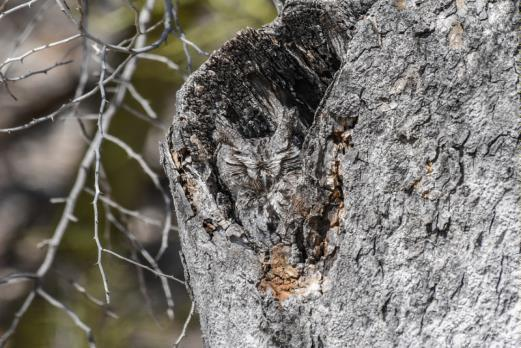
\includegraphics[scale=0.25]{COD_Zh_translate/figures/example1.png}
        \hspace{5mm} %调整纵向距离
    \end{minipage}
}
\subfigure
{
 	\begin{minipage}[htbp]{.18\linewidth}
        \centering
        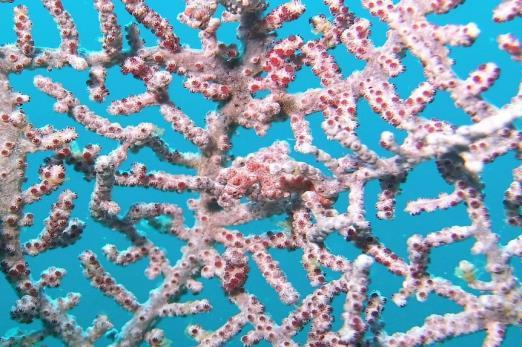
\includegraphics[scale=0.25]{COD_Zh_translate/figures/example2.png}
        \hspace{5mm} %调整纵向距离
    \end{minipage}
}
\subfigure
{
 	\begin{minipage}[htbp]{.18\linewidth}
        \centering
        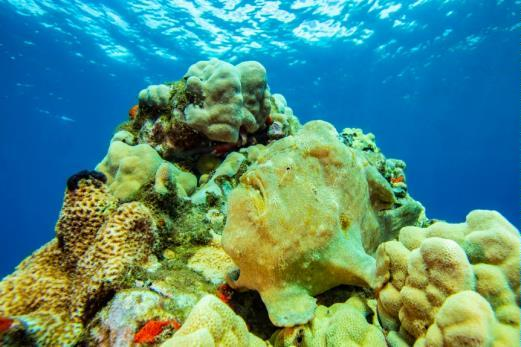
\includegraphics[scale=0.25]{COD_Zh_translate/figures/example3.png}
        \hspace{5mm} %调整纵向距离
    \end{minipage}
}
\subfigure
{
 	\begin{minipage}[htbp]{.18\linewidth}
        \centering
        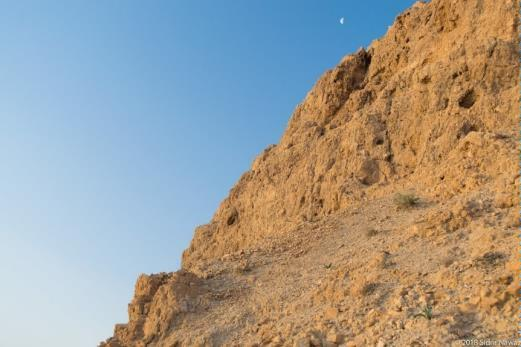
\includegraphics[scale=0.25]{COD_Zh_translate/figures/example4.png}
        \hspace{5mm} %调整纵向距离
    \end{minipage}
}
\subfigure
{
 	\begin{minipage}[htbp]{.18\linewidth}
        \centering
        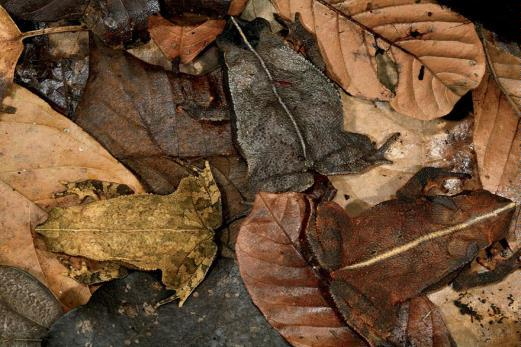
\includegraphics[scale=0.25]{COD_Zh_translate/figures/example5.png}
        \hspace{5mm} %调整纵向距离
    \end{minipage}
}
\caption{COD10K 数据集示例图。你能找到隐藏在图片中的伪装物体吗?以彩色电子版阅览时视觉效果最佳。 答案见补充材料。}
\label{fig:COD10K_examples}
\end{figure*}


%%%%%%%%% ABSTRACT%%%%%%%%%%%
\begin{abstract}
伪装物体检测(Camouflaged Object Detection, COD),顾名思义,旨在识别“无缝”嵌入其周围环境 的物体,本文对这项新任务展开了全面的研究。与传 统的物体检测相比,通常伪装物体与其背景之间具 有高度相似性,因此伪装物体检测更具挑战。为解决 这一问题,本文精心构建了 COD10K 数据集,它包 含了 10,000 张图像,且涵盖了各种自然场景,具有超过78个类别的伪装物体。所有的图像都进行了稠密的标注,包括类别、包围盒、对象级/实例级,以及抠图级的标签。COD10K 数据集可以助力许多视觉任务,例如目标定位、图像分割和抠图技术等。同时, 本文也为伪装物体检测任务提供了一个简单且有效 的框架,称为搜索识别网络(Search Identification Network,SINet)。没有借助过多技巧,SINet 在所有 数据集上的表现均优于其它先进的物体检测基准模 型。因此,SINet 是一个鲁棒的、通用的架构,这有助 于促进伪装物体检测的发展。最后,通过对 13 种最 先进模型进行系统评估,本文给出了许多有趣的发 现并且展示了一些伪装物体检测的潜在应用。希望 本文的研究能为这一新领域的学者提供更多探索机 会。详见:https://github.com/DengPingFan/SINet/
\end{abstract}



%%%%%%%%% BODY TEXT %%%%%%%%%%%%%%%%%%%%%%%%%%%%%%%%%%%%%%%%
\section{引言}\label{sec:Introduction}
你能在\figref{fig:COD10K_examples}中找到伪装的物体吗?生物学家将
这类伪装方式称为背景匹配,即动物为避免被识别 [49],会尝试改变其自身颜色以“完美”地融入周围 环境。感官生态学家的研究表明,这种伪装策略是通 过欺骗观察者的视觉感知系统而产生的 [58]。因此, 解决伪装物体检测(Camouflaged Object Detection COD)任务需要大量的视觉感知知识 [61]。

\begin{figure}[h!]
  \begin{overpic}[width=\columnwidth]{Comparison_COD.png} \small
  \put(6,-4){(a)原图}
  \put(26,-4){(b)通用物体}
  \put(52,-4){(c)显著物体}
  \put(76,-4){(d)伪装物体}
    \end{overpic}\\
    \caption{给定一张输入图像(a),(b)为全景分割 [31] 的真值(全景分割检测中的通用物体 [40,45]包括stuff和things),(c)是显著实例/物体检测 [17, 34, 62, 77](检测最吸引人注意力的目标),(d)是本文提出的伪装物体检测任务,即检测出与 周围环境具有相似模式(例如边缘,纹理或颜色)的物体。如 图所示,两只蝴蝶的边缘与香蕉融合在一起,难以识别。
    }\label{fig:Comparsion_COD_SOD}
\end{figure}

如\figref{fig:Comparsion_COD_SOD}所 示,物体物与背景之间高度的相似性使 COD 远比 传统的显著物体检测(SOD)[1, 5, 18, 26, 63–67, 69] 或通用物体检测(GOD)[4,80] 更具挑战性。
除了其学术价值外,伪装物体检测还有助于推 动下列领域的实际应用:计算觉领域(可用于搜索 和救援工作,或寻找稀有物种)、医学图像分析领域
(如息肉分割 [15] 和肺炎分割 [19,68])、农业领域 (如蝗虫入侵监控)和艺术领域(用于真实感图像融
合 [22] 或艺术消遣 [6])。
目前,由于缺乏规模足够大的数据集,伪装物体检测的研究还不够深入。为了对 COD 课题进行
全面的研究,本文做出了两项
贡献。首先,本文专门 为COD任务精心构建了COD10K 数据集。它与 现有的数据集有以下方面的区别:
\begin{itemize}
    \item COD10K 数据集包含了1万张图像,涵盖了78 种伪装物体类别,属于水生、飞行、两栖和 陆地等。
    \item 所有的伪装图像都赋予了不同的层级标签,如 类别、包围盒、对象级和实例级。这些标签会使 得许多视觉任务受益,如目标定位,似物性检测,语义边缘检测 [43],任务迁移学习 [70] 等。
    \item 每张伪装图像都加上了真实环境中遇到的具有 挑战的属性以及抠图级 [74](标注一张图像耗时 约 60 分钟)的标签。这些高质量的标注有助于 对算法性能进行更深入的分析。
\end{itemize}%让文本空两行就能做到下一段、缩进


其次,使用本文构建的 COD10K 数据集和两个 现有数据集 [33,57],来共同构成最大的伪装物体检 测训练数据集,对 13 种最先进 (SOTA) 的基准模型 [3,24,28,33,36,39,41,52,69,76,78,79,83] 进行严格 的评估。本文的评估成为了目前最大规模的 COD 研 究。此外,本文还提供了一个简单而有效的框架,名 为 SINet (Search Identification Net)。值得注意的 是,SINet 的训练总时长仅为 1 小时左右,并且在目 前所有 COD 数据集上都达到了 SOTA 的性能。这 表明 SINet 可能是解决 COD 问题的潜在方案。在 深度学习时代下,本文是第一个完整的 COD 任务 评测,同时以伪装的角度去重新理解物体检测任务。





%%%%%%%%%%%%%%%%%%%%%%%%%%%%%%%%%%%%%%%%%%%%%%%%%%%%%%%%%%%%%%%%%%%%%%%%%%%%%%%%%
\begin{figure*}[tp]
    \centering
    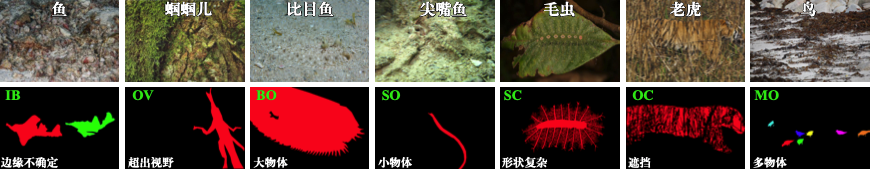
\includegraphics[width=0.95\textwidth]{COD_Zh_translate/figures/COD10K_features.png}
    \caption{COD10K 数据集中各式各样的具有挑战性的属性示例图。属性表详见\tabref{tab:COD_Dataset}。以彩色电子版阅览视觉效果最佳。}
    \label{fig:COD10K_features}
\end{figure*}

\section{相关工作}
\label{sec:RelatedWorks}
根据 [80] 的研究,物体大致可以分为三类:通 用物体、显著物体和伪装物体。接下来本文将逐一介绍这些检测策略。
\subsection{通用物体和显著物体检测}
\mypara{通用物体检测(Generic Object Detection, COD)} 通用物体检测是计算机视觉中最热门的方向之一 [11,31,38,56]。值得注意的是,通用物体既可以 是显著的也可以是伪装的;伪装物体可视为通用物 体中较难的特例(如图. 9中第二行和第三行)。典型 的 GOD 任务包括语义分割和全景分割(见\figref{fig:Comparsion_COD_SOD} b)。
\mypara{显著物体检测(Salient Object Detection, SOD)}SOD 旨在识别图像中最引人注意的物体,然后对其 轮廓进行像素级分割 [29,39,73,78]。虽然“显著”一 词本质上与“伪装”相反(突出与浸入),但是显著 物体也可以为伪装物体检测提供重要信息,即可以 把包含显著对象的图像作为伪装物体检测的负样本。
\begin{table}
    \scalebox{0.57}{
    \centering
    \begin{tabular}{c|ccc|ccccccc}
\hline
数据集 & 年份 & 数量 & 类 & Att. & Bbox. & MI. & Ins. & Cate. & Spi. & Obj. \\ \hline
CHAMELEON{[}57{]} & 2018 & 76   & -  &      &       &     &      &       &      & \checkmark    \\
CAMO{[}33{]}      & 2019 & 2.5k & 8  & \checkmark    &       &     &      &       & \checkmark    & \checkmark    \\ \hline
COD10K(Ours)      & 2020 & 10k  & 78 & \checkmark    & \checkmark     & \checkmark   & \checkmark    & \checkmark     & \checkmark    & \checkmark    \\ \hline
\end{tabular}
    }
    \caption{从 COD 数据集对比信息来看,COD10K 数据集提 供了更丰富的注释标签。数量(Img.):图片数。类(Cls.): 类别。Att.:属性。BBox.;包围盒。Ml.:抠图 [74] 级标注
(图. 7)。Ins.:实例级标签。Cate.:类别标签。Spi.:显式拆 分训练集与测试集。Obj.:物体。}\label{tab:COD_Dataset}
\end{table}



\subsection{伪装物体检测}
伪装物体检测在生物学、艺术、医学等领域有着悠久而丰富的历史,对提高人类的视觉感知能力影 响巨大。Abbott Thayer[59]和 Hugh Cott[8]的关于伪装动物的两项杰出研究至今仍然影响广泛。感 兴趣的读者可以仔细阅读 Stevens等人[58]关于这段历史的描述。\mypara{数据集}CHAMELEON [57] 是一个未经同行评议的 数据集,仅包含 76 张图像,手工标注了对象级的真 值图(GTs)。这些图像是以“伪装的动物”为关键 字,通过谷歌搜索引擎收集的。另一个同期数据集 称为 CAMO [33],它具有 2500 张图像 (其中 2000 张用于训练,500 张用于测试),涵盖了八个类别。它 的两个子集 CAMO 和 MS-COCO,分别包含 1250 张图像。


不同于现有数据集,COD10K 数据集旨在提供一个更具挑战性,质量更高并且稠密标注的数据集。 COD10K 是迄今为止最大的伪装物体检测数据集, 包含有 1 万张图像(6000 张用于训练,4000 张用于 测试)。详见\tabref{tab:COD_Dataset}
\begin{figure*}
    \centering
    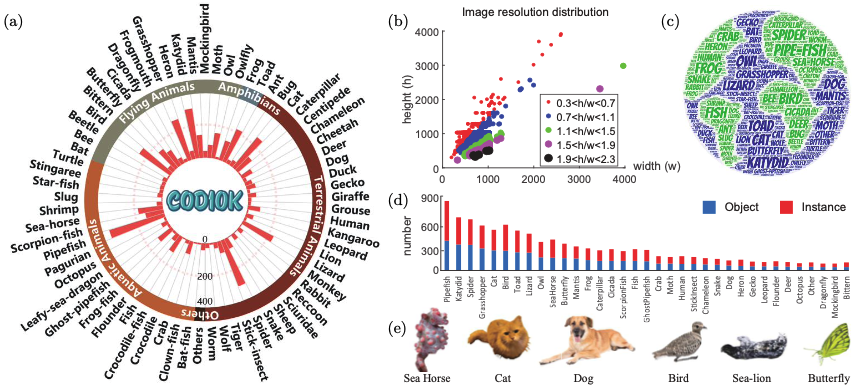
\includegraphics[width=0.95\textwidth]{COD_Zh_translate/figures/Catagory_COD10k.png}\small
    \caption{COD10K 数据集的统计信息和伪装类别示例。(a) 分类系统及其直方图分布。(b) 图像分辨率分布。(c) 词云分布。(d) 对象/实例的类别数量。(e) 子类示例。}
    \label{fig:Catagory_COD10k}
\end{figure*}
%这几段有大问题,很多数学公式里的符号都没有正常输入出来
\mypara{伪装的类型}伪装图像大致可分为两类,自然伪装和人工伪装的图像。动物 (例如昆虫、头足类动物) 的 自然伪装是一项生存技能,用来防止被捕食者识别。 相比之下,人工伪装通常被应用于视频监控环境;也 会出现在产品的生产过程中 (即产品缺陷检测);或 者在游戏或艺术中用来隐藏信息。
\mypara{COD定义} 和类别相关的语义分割任务不同,COD 任务与类别无关。因此,COD 任务简单且容易定义。 输入一张图像,通过伪装物体检测方法,为每个像 素i分配置信度pi ∈[0,1],其中pi 表示像素i的 概率值。0 表示此像素不属于伪装物体,而 1 则表 示完全属于伪装物体。本文主要研究对象级的 COD 任务,实例级 COD 作为未来的工作。
\mypara{评估指标}平均绝对误差(Mean absolute error, MAE)已被广泛用于 SOD 任务。和 Perazzi 等 人 [50] 一样,本文也使用了平均绝对误差 M 指 标(MAE(M))来评估预测图像 C 和真值图像G之间的像素级精度。尽管 MAE 指标能有效地评估错 误的出现和数量,但它不能评估错误出现的位置。最 近,范等人提出了一种基于人类视觉感知机制的增 强-匹配评价指标(E-measure,Eφ )[13],它同时考虑了像素级信息的匹配和图像级信息的统计。该评价 指标显然适用于评估伪装物体检测结果的整体和局 部精度。由于伪装物体通常包含复杂的形状,COD 还需要一个可以判断结构相似性的评价指标,因此 本文引入了 S 测评法(S-measure,Sα)[12]。最新 研究 [12,13] 表明,加权的 F 测评法(F-measure, Fβw )[44] 比传统的 Fβ 评测法更可靠。因此,本文 也在 COD 领域中使用这一评估指标。
%%%%%%%%%%%%%%%%%%%%%%%%%%%%%%%%%%%%%%%%%%%%%%%%%%%%%%%%%%
\section{文本数据集}\label{sec:HC}
新任务和数据集 [7,11,37,48,82] 的出现促进了 计算机视觉各个领域的快速发展。例如,ImageNet [53] 数据集的出现使得深度模型在视觉识别任务上 成为了可能。本文构建 COD 数据集的初衷与之相 似,是为了:(1) 提供一项新的具有挑战性的任务, (2) 促进对新主题的研究,(3) 激发新想法。\figref{fig:COD10K_examples}、\figref{fig:COD10K_features}以及\figref{fig:Catagory_COD10k} (e)为 COD10K 的示例。接下来, 本文从以下三个方面详细阐述 COD10K 数据集。
\subsection{图像收集}
根据 [18,51] 的研究,数据集的标注质量和规 模决定了基准数据集的时间长短。为了延长其寿命, COD10K 数据集包含 10,000 张图像(5,066 张伪装 图像,3,000张背景图像,1,934张无伪装的图像),包含 10 个超类和 78 个子类(69 个伪装类,9 个非 伪装类),这些图像来源于多个摄影学网站。
大多数伪装图像来自 Flickr 网站,搜索关键字 为:camouflaged animal, unnoticeable animal, cam- ouflaged fish, camouflaged butterfly, hidden wolf spi- der, walking stick, dead-leaf mantis, bird, sea horse, cat, pygmy seahorses 等 (见\figref{fig:Catagory_COD10k} e),这些图像仅应 用于学术研究。其它伪装图像(约 200 张)来自下列 网站,如:Visualhunt,Pixabay,Unsplash,Free- images 等,这些图片不受版权和付费约束。为了避 免选择偏见 [18],我们还从 Flickr 收集了 3,000 张 显著图像。为了进一步丰富负样本,又从互联网上 下载了 1,934 张无伪装的图像,包括森林、雪地、草 地、天空、海水和其他类别的场景。有关图像选择方 案的更多信息,请见周等人的研究 [81]。

\begin{figure}[tp]
    \centering
    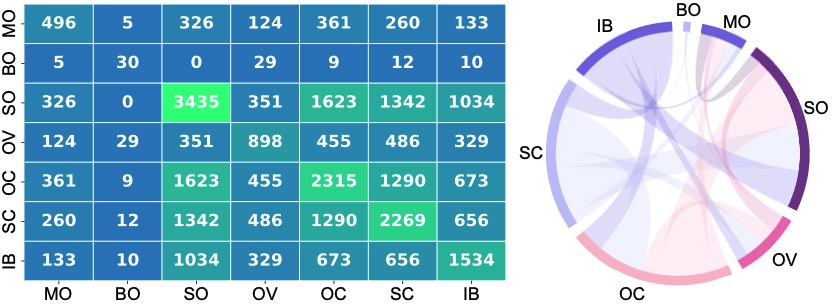
\includegraphics[width=0.98\columnwidth]{COD_Zh_translate/figures/Inter_relation_COD10k.png}\small
    \caption{COD10K 左图:COD10K 数据集的共生属性分布。网格中的数字为图像总数。右图:属性间的相互依赖关系。弧长越长则两属性间的相关性就越高。}
    \label{fig:Catagory_COD10k}
\end{figure}

\begin{table}
    \scalebox{0.78}{
    \centering
    \begin{tabular}{cl}
        \hline
        属性 & 描述                                                                                          \\ \hline
        MO & 多物体 图像至少包含两个物体\\
        BO & 大物体 物体面积和图像面积的比值大于等于 0.5\\
        SO & 小物体 物体面积和图像面积的比值小于等于 0.1\\
        OV & 超出视野 物体的部分区域超出了图像边界\\
        OC & 遮挡 物体被部分遮挡。\\
        SC & 形状复杂 物体包含细小部分 (如:动物脚).\\
        IB & \begin{tabular}[c]{@{}l@{}}边缘不确定 目标周围区域的前景和背景具有相似的颜色 \\ (与RGB直方图χ2的距离τgc小于0.9)\end{tabular} \\ \hline
        \end{tabular}
            }
    \caption{属性描述 (示例见\figref{fig:COD10K_features})。}\label{tab:COD_Dataset}
\end{table}
\subsection{专业标注}
最新公布的数据集 [10, 16, 17] 表明,在创建大 规模数据集时,建立分类系统至关重要。受 [46] 启 发,本文进行了分层标注(采用众包方式标注)(类别$\longrightarrow$包围盒$\longrightarrow$属性$\longrightarrow$对象/实例)。
\begin{itemize}
    \item 类别. 如图. 4(a)所示,首先创建五个超类。 然后从收集到的数据中归纳了 69 个最常见的子类。 最后,标注每个图像的子类和超类。如果候选图像 不属于任何已有类别,则将其归为“其他”类。
    \item 包围盒. 为了将COD10K数据集扩展到伪装物采样(proposal)任务,本文还细致地为每张图像 标注包围盒。
    \item 属性. 与文献 [18,51] 保持一致,本文采用自 然场景中常见的极具挑战的属性 (如遮挡、边缘不确 定),来标注每张图像。表. 2提供了属性描述,\figref{fig:Catagory_COD10k}展示了共生属性分布情况。
\end{itemize}
%%%%%%%%%%%%%%%%%%%%%%%%%%%%%%%%%%%%%%%%%%%%%%%%%%%%%%%%%%%%%%%%这块的三个图是非常值得玩味的
%第一张图因为放在subsection3.3上面,不形成破坏,直接使用[tp]就上去了
%第2、3张图都是破坏的subsection3.3,所以可以放在这个subsection前面,然后统一自动排版
%如果最后一张图放置在subsection结束之后,很有可能又会单独成页
%%%%%%%%%%%%%%%%%%%%%%%%%%%%%%%%%%%%%%%%%%%%%%%%%%%%%%%%%%%%%%%
\begin{figure}[tp]
    \centering
    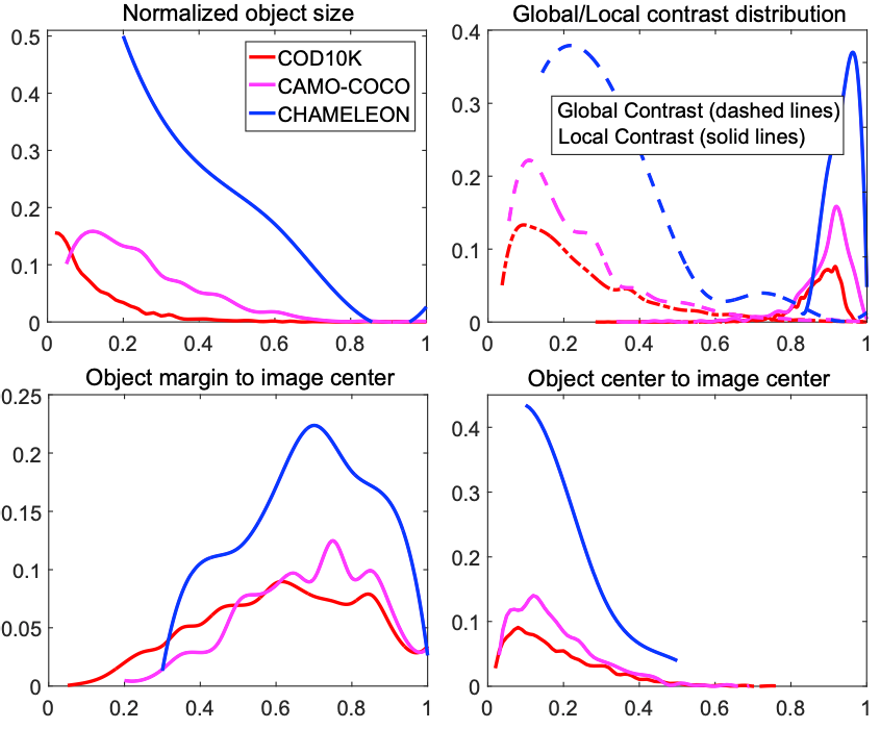
\includegraphics[width=0.98\columnwidth]{COD_Zh_translate/figures/Graph_analyse_COD10k.png}\small
    \caption{ COD10K 数据集与现有 COD 数据集相比,它包含小 物体(左上),包含更复杂的伪装(右上)并且受中心偏差影 响更小(左下/右下)。
}
    \label{fig:Graph_analyse_COD10k}
\end{figure}

\begin{figure}[bp]
    \centering
    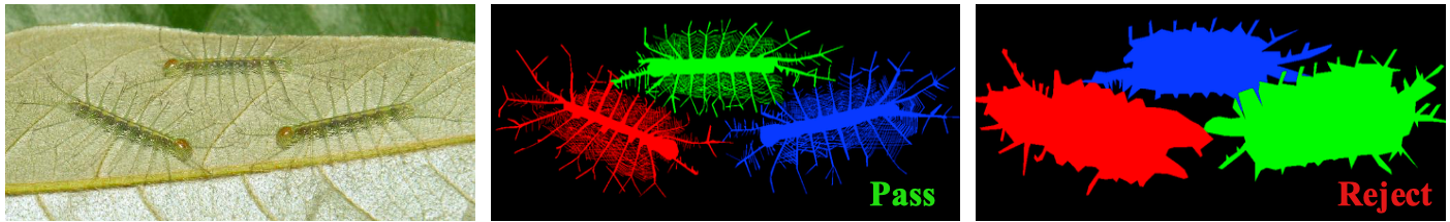
\includegraphics[width=0.98\columnwidth]{COD_Zh_translate/figures/High_quality.png}\small
    \caption{ 高质量的抠图级标注 [74]。
}
    \label{fig:High_quality}
\end{figure}
%尤其是这张图的摆放位置,十分有参考价值
\begin{figure*}[t]
    \centering
    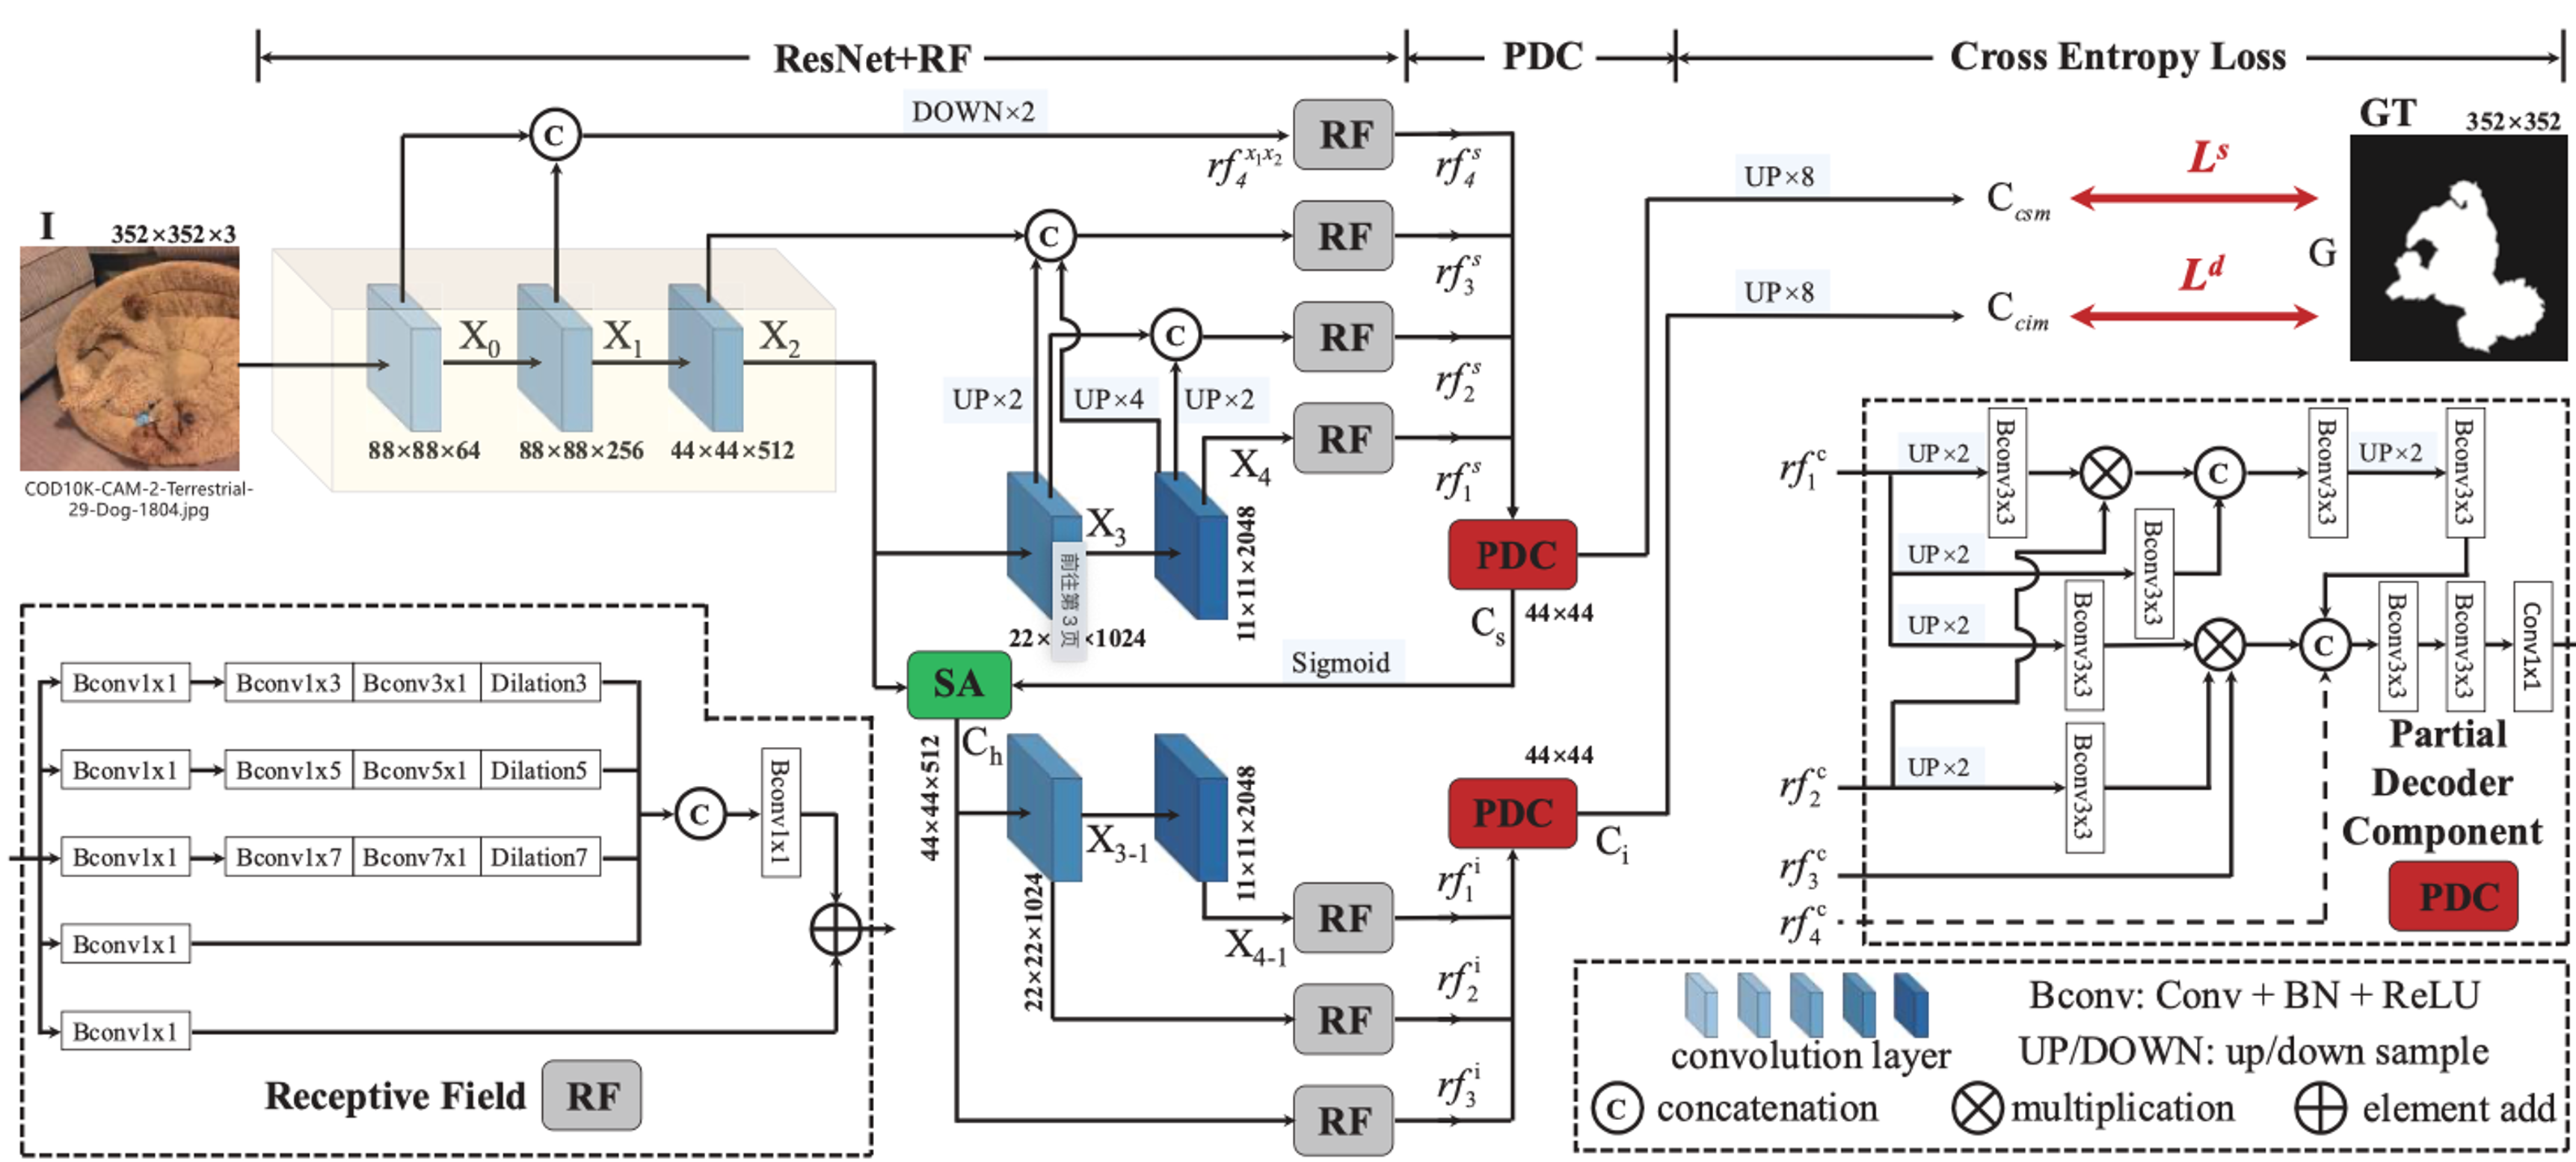
\includegraphics[width=0.98\textwidth]{COD_Zh_translate/figures/SINet_Struct.png}\small
    \caption{ SINet框架概要。本框架主要包括两个部分:感受野 (RF) 的感受野结构。PDC模块再现了动物捕食的搜索和识别阶段。SA和部分解码组件(PDC).RF模块用来模拟人类视觉系统中 为 [69] 中描述的搜索注意函数。详见 § 4。}
    \label{fig:SINet_Struct}
\end{figure*}

\subsection{数据集特点与统计信息}
\begin{itemize}
    \item 物体大小. 根据 [18] 的研究,在图. 6(左上 角)中绘制了归一化的物体尺寸,分布从 0.01\%到 80.74\%(平均:8.94\%)。与 CAMO-COCO、CPD1K 和 CHAMELEON 相比,本文数据集具有更广的尺寸范围。
    \item 全局/局部对比度. 为了考察物体是否容易检 测,本文使用全局与局部比值评估方法 [35]。图. 6(右 上角) 表明了 COD10K 数据集比其他数据集更具挑 战性。
    \item 中心偏见. 由于人类会自然地将注意力集中在场景中心,因此摄影时就会产生这样的偏见。本 文采用 [18] 中的策略来分析这种偏见。图. 6(底部) 表明了本文数据集受到的中心偏见的影响更小。
    \item 质量控制. 为了确保高质量的标注,标记过程 邀请了三位观察者参与,并进行 10 组的交叉验证。 图. 7展示了通过和拒绝的标注示例。每张图像的实 例级标注平均耗时 60 分钟。
    \item 超类和子类的分布. COD10K 包括 5 个超类 (陆地生物、空中生物、水生生物、两栖动物以及其 他类)和 69 个子类(例如:蝙蝠鱼, 狮子, 蝙蝠, 青 蛙等),各类别的词云和对象/实例数量的示例分别显示在图. 4 c 和 d 中。
    \item 分辨率分布. [71] 研究表明,高分辨率图像可
以为模型训练提供更多物体边缘的细节从而在测试 时获得更好的性能。图. 4 (b)展示了 COD10K 数 据集图像分辨率的分布情况,它含有大量的 1080p 全高清图像。
    \item 数据集划分. 为了给深度学习模型提供大量 的训练数据,本文将 COD10K 数据集划分为:6,000 张图像的训练集和 4,000 张图像的测试集,图像分 别从每个子类中随机选择。
\end{itemize}

\section{本文框架}
\mypara{动机}生物学的研究 [23] 表明,捕食者在狩猎时,首 先会判断是否存在潜在猎物,即搜索猎物;然后,目 标动物被识别;最后,动物被捕获。
\mypara{概述}本文的 SINet 框架受到狩猎过程的前两阶段 的启发。框架主要包括两个模块:搜索模块 (Search Module, SM) 和识别模块 (Identification Module, IM)。前者 (§ 4.1) 负责搜索被伪装的物体,而后者 (§ 4.2) 则用于精确检测物体。


\subsection{搜索模块(Search Module,SM)}
神经科学实验已证实,在人类视觉系统中,一组多尺度的群感受野(population Receptive Fields,pRFs)有助于让靠近视网膜中央凹的区域更加显著,而该区域对小的空间位移非常敏感[42]。于是,本文在搜索阶段(通常是在较小的、局部空间中)使用 RF [42,69] 模块来整合更具鉴别性的特征表示。具 体而言,对于输入图像 I ∈ RW×H×3 ,可利用 ResNet- 50 [25] 模型提取出一组特征{Xk}4k=0。为了保留更多信息,本文将第二层特征层的步长参数设置为1, 使其和输入图像具有相同的分辨率。因此,每一层 分辨率为{[Hk,Wk ],k = 4,4,8,16,32} 。
最新研究 [79] 显示,更浅的卷积层中的低级
特征保留了用于构建物体边缘的空间信息,而深层
的深层卷积层的特征保留了用于定位目标的语义信
息。由于神经网络本身的固有的特性,本文将提取
的特征进行分层:低层 {X0, X1},中层 X2 和高层
{X3, X4},并通过拼接、上采样和下采样等操作进行
组合。与 [79] 不同,本文的 SINet 采用稠密连接策
略 [27] 来保存来自不同特征层的更多信息,然后使
用改进的 RF [42] 组件来扩大感受野。例如,先使用
拼接操作来融合低级特征 {X0, X1},然后将分辨率
下采样为原始一半。再将融合后的新特征 rf x1x2 进 4
一步输入到 RF 组件生成 rf4s 特征。如图. 8所示,在
组合了三个层次的特征之后,得到了一组增强的特 征 {rfks, k = 1, 2, 3, 4},用于鲁棒地学习伪装线索。 感受野 (Receptive Field, RF). RF 模块包括五 个分支 {bk, k = 1, . . . , 5}。在每个分支中,第一个 卷积层 (Bconv) 的尺寸为 1 × 1,用以将通道数降为 32。其后两层分别为:(2k − 1) × (2k − 1) Bconv 层 和3×3Bconv层。当k>2时,空洞卷积率设置为 (2k − 1)。前四个分支串联后,通过 1 × 1 Bconv 操 作,其通道数降为 32。最后,加入第 5 个分支,并 整体输入进 ReLU 函数以获得特征 rfk。


\subsection{识别模块 ((Identification Module, IM)}
%%%%%%%%%%%%%%%%%%%%%%%%%%%%%%%%%%%%%%%%%%%%%%%%%%%%%%%%%%%%%%%%%%%%%%
\section{实验比较}\label{sec:Experiment}



%%%%%%%%%%%%%%%%%%%%%%%%%%%%%%%%%%%%%%%%%%%%%%%%%

\section{总结与展望}\label{sec:Conclusion}



%引文我就只能意思一下了,COD原文引用太多了,我这边随便找齐了百多篇放到了bib里面,然后到时候我只能说随便引了,最后用goodnotes弄一下pdf

% {\small
% \bibliographystyle{ieee}
% \bibliography{COD_fake}
% }

% \end{CJK*}
\end{document}
